\usetikzlibrary{decorations.pathreplacing}
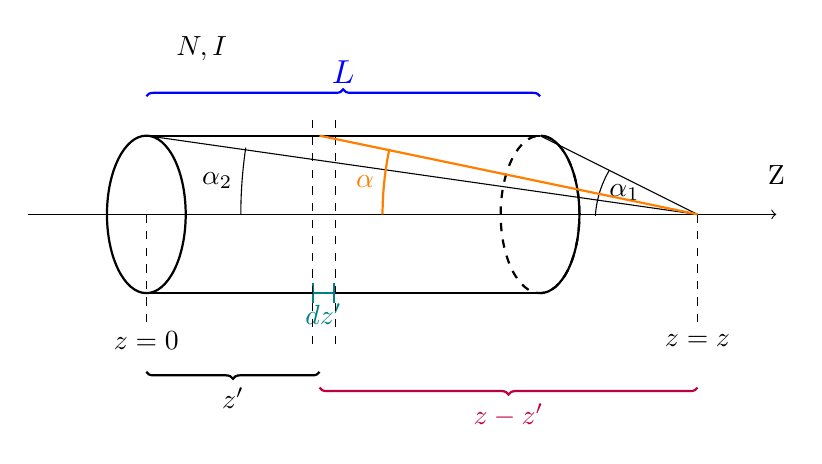
\begin{tikzpicture}
\draw [thick] (3.5,0) node (v1) {} ellipse (0.5 and 1);
\draw [fill, white] (2.5,1.5) rectangle (3.5,-1.5);
\draw [thick] (-1.5,0) ellipse (0.5 and 1);
\draw [thick](-1.5,1) -- (3.5,1) (-1.5,-1) -- (3.5,-1);
\draw [thick][dashed] (v1) ellipse (0.5 and 1);
\draw [->, thin] (-3,0) -- (6.5,0);
\node at (6.5,0.5) {Z};
\draw [decorate,decoration=brace,draw=blue, thick] (-1.5,1.5) -- (3.5,1.5) node [blue,midway, above, scale=1.2]{$L$};
\draw (3.5,1) -- (5.5,0);
\draw (4.2026,-0.0184) arc (176.4011:149.4:1.3) node [right, midway]{$\alpha_1$};
\draw (-1.5,1) -- (5.5,0);
\draw (-0.3,0) arc (180:171.6:5.8)node [left, midway]{$\alpha_2$};
\node at (-0.8,2.1) {$N,I$};
\node at (-1.5,-1.6) {$z=0$};
\draw [dashed](-1.5,0) -- (-1.5,-1.4);
\draw [|-|, thick, teal](0.6,-1) -- (0.9,-1) node [below, midway]{$dz'$};
\draw [dashed, ultra thin](0.6,1.2) -- (0.6,-1.7);
\draw [dashed, ultra thin](0.9,1.2) -- (0.9,-1.7);
\draw [dashed](5.5,0) -- (5.5,-1.4);
\node at (5.5,-1.6) {$z=z$};
\draw [orange, thick](0.7,1) -- (5.5,0);
\draw [orange, thick](1.5,0) arc (180:168:4)node [left, midway]{$\alpha$};
\draw [decorate,decoration=brace, thick](0.7,-2) -- (-1.5,-2)node [below=2, midway]{$z'$};
\draw [decorate,decoration=brace, thick, purple](5.5,-2.2) -- (0.7,-2.2)node [below=2, midway]{$z-z'$};
\end{tikzpicture}